%%%%%%%%%%%%%%%%%%%%%%%%%%%%%%%%%%%%%%%%%
% University/School Laboratory Report
% LaTeX Template
% Version 3.1 (25/3/14)
%
% This template has been downloaded from:
% http://www.LaTeXTemplates.com
%
% Original author:
% Linux and Unix Users Group at Virginia Tech Wiki 
% (https://vtluug.org/wiki/Example_LaTeX_chem_lab_report)
%
% License:
% CC BY-NC-SA 3.0 (http://creativecommons.org/licenses/by-nc-sa/3.0/)
%
%%%%%%%%%%%%%%%%%%%%%%%%%%%%%%%%%%%%%%%%%

%----------------------------------------------------------------------------------------
%	PACKAGES AND DOCUMENT CONFIGURATIONS
%----------------------------------------------------------------------------------------

\documentclass{article}

\usepackage[version=3]{mhchem} % Package for chemical equation typesetting
\usepackage{siunitx} % Provides the \SI{}{} and \si{} command for typesetting SI units
\usepackage{graphicx} % Required for the inclusion of images
\usepackage{natbib} % Required to change bibliography style to APA
\usepackage{amsmath} % Required for some math elements 
\usepackage{enumerate} % Required for the enumerate function
\usepackage[americanvoltages,siunitx]{circuitikz} % Required for the drawing of circuit diagrams
\usepackage{caption}
\usepackage{graphicx}
\usepackage{subcaption}
\usepackage{xfrac}
\usepackage{float}
\usepackage{enumitem}
\usepackage{enumerate}
\usepackage{amssymb}

\setlength\parindent{0pt} % Removes all indentation from paragraphs

\renewcommand{\labelenumi}{\alph{enumi}.} % Make numbering in the enumerate environment by letter rather than number (e.g. section 6)

%\usepackage{times} % Uncomment to use the Times New Roman font

%----------------------------------------------------------------------------------------
%	DOCUMENT INFORMATION
%----------------------------------------------------------------------------------------

\title{Electrical Circuit Analysis \\ Assignment 2 \\ ENG223} % Title

\author{Shane \textsc{Reynolds}} % Author name

\date{\today} % Date for the report

\begin{document}

\maketitle % Insert the title, author and date

\begin{center}
\begin{tabular}{l r}
Instructor: & Dr Kamal Debnath % Instructor/supervisor
\end{tabular}
\end{center}

% If you wish to include an abstract, uncomment the lines below
% \begin{abstract}
% Abstract text
% \end{abstract}

%----------------------------------------------------------------------------------------
%	SECTION 1
%----------------------------------------------------------------------------------------

\section*{Assignment 2.1}

The diagram of the circuit is as follows:
\begin{center}
	\begin{circuitikz}
		\draw (0,0)
		to [sV, l=$E_f$] (0,2)
		to [L, l=$jX_s$] (3,2)
		to [short, o-] (4,2)
		to [generic, l=Load] (4,0)
		to [short, -o] (3,0)
		to [short] (0,0)
		;
		
		\draw (3.5,2)
		to [open, v=$V_t$] (3.5,0)
		(1.5,1) node[scale=4]{$\circlearrowright$}
		(1.5,1) node{$I_L$}
		;
		
	\end{circuitikz}
\end{center}


We are not told what the load is comprised of, only that the current $I_L$ lags the voltage $V_t$ by some unspecified angle. This leaves us unable to determine what the phasor diagram for the voltage and current look like. One possible example is as follows:

\begin{center}
	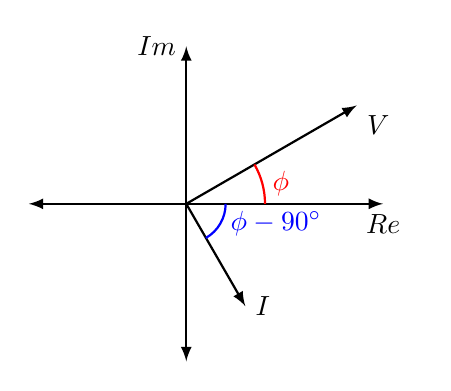
\begin{tikzpicture}[>=latex]
	\draw[style=help lines] (0,0) (3,2);
	
	\coordinate (vec1) at (300:1.5); 
	\coordinate (vec2) at (30:2.5);
	\coordinate (vec3) at (0:2.5);
	\coordinate (vec4) at (90:2);
	\coordinate (vec5) at (270:2);
	\coordinate (vec6) at (180:2);
	
	\draw[->,thick,black] (0,0) -- (vec1) node[right] {$I$};
	\draw[->,thick,black] (0,0) -- (vec2) node[below right] {$V$};
	\draw[->,thick,black] (0,0) -- (vec3) node [below] {$Re$};
	\draw[->,thick,black] (0,0) -- (vec4) node [left] {$Im$};
	\draw[->,thick,black] (0,0) -- (vec5);
	\draw[->,thick,black] (0,0) -- (vec6);
	
	\draw [red, thick] (1.0,0) arc [start angle=0, end angle=30, radius=1cm]
	node [midway, right] {$\phi$};    
	
	\draw [blue, thick] (0.5,0) arc [start angle=0, end angle=-60, radius=0.5cm]
	node [midway, right] {$\phi-\ang{90}$};    
	\end{tikzpicture}
\end{center}

In this example, it is clear that the current lags the voltage by 90$\si{\degree}$.

\newpage
%----------------------------------------------------------------------------------------
%	PROBLEM 2
%----------------------------------------------------------------------------------------

\section*{Assignment 2.2}

\begin{enumerate}
	
	\item
		In any circuit system, power is conserved. Hence, it must be true that the power delivered by the source, $S_{source}$, is equal to the power dissipated by the $\Delta$-load plus the power dissipated by the $Y$-load. That is:
		
		\begin{align*}
			S_{source} = S_\Delta + S_Y
		\end{align*}
		
		Now, rearranging the above we get:
		
		\begin{align*}
			S_\Delta &= S_{source} - S_Y \\
		\end{align*}
		
		We are told that the power factor for the source is 0.75 lagging, hence the phase angle is given by:
		
		\begin{align*}
			\theta_{source} &= \arccos(powerfactor_{source}) \\
			&= \arccos(0.75) \\
			&= 41.41\si{\degree}
		\end{align*}
		 
		The power factor for the $Y$-connected load is 0.6 lagging, hence the phase angle is given by:
		
		\begin{align*}
			\theta_{Y} &= \arccos(powerfactor_{Y}) \\
			&= \arccos(0.6) \\
			&= 53.13\si{\degree}
		\end{align*}
	
		Using the phase angles, we can now solve for the power dissipated from the $\Delta$-load:
		
		\begin{align*}
			S_\Delta &= 14000 \angle 41.41\si{\degree} - 9000 \angle 53.13\si{\degree} \\
			&= 14000 \cos(41.41\si{\degree}) + j14000 \cos(41.41\si{\degree}) - [9000 \cos(53.13\si{\degree}) + j9000 \sin(53.13\si{\degree})] \\
			&= 5099.93 + j2060.21 \\
			&= 5500.34 \angle 22 \si{\degree} \si{VA}
		\end{align*}
		
		Now, we know that the power per phase is one third of the total power dissipated by the $\Delta$-connected load, hence:
		
		\begin{align*}
			S_{\Delta/\phi} &= \frac{S_\Delta}{3} \\
			&= \frac{5500.34 \angle 22 \si{\degree}}{3}
		\end{align*}
		
		Hence the complex power per phase for the $\Delta$-connected load is:
		
		\begin{align*}
			S_{\Delta/\phi} = 1833.45 \angle 22 \si{\degree} \si{VA}
		\end{align*}
	
	\item
		For a positive sequenced, balanced three phase $Y$-connected load, we know that:
		
		\begin{align*}
			\boldsymbol{V_{AB}} = \sqrt{3}\angle 30 \si{\degree} \times \boldsymbol{V_{AN}}
		\end{align*}
		
		Now, to find $\boldsymbol{V_{AN}}$ we use the power formula:
		
		\begin{align*}
			\boldsymbol{S_\phi} = \boldsymbol{V_\phi} \times \boldsymbol{I_\phi^*}
		\end{align*}
		
		The complex power per phase in the $Y$-connected load is given by:
		
		\begin{align*}
			\boldsymbol{S_\phi} &= \frac{\boldsymbol{S_Y}}{3} \\
			&= \frac{9000 \angle 53.13 \si{\degree}}{3} \\
			&= 3000 \angle 53.13 \si{\degree} \si{VA}
		\end{align*}
		
		Hence, rearranging the above formula we find that the phase voltage at the $Y$-connected load is given by:
		
		\begin{align*}
			\boldsymbol{V_\phi} &= \frac{\boldsymbol{S_\phi}}{\boldsymbol{I_\phi^*}} \\
			&= \frac{3000 \angle 53.13 \si{\degree}}{10 \angle 30 \si{\degree}} \\
			&= 300 \angle 23.13 \si{\degree} \si{\volt}
		\end{align*}
		
		Finally, we find the line voltage:
		
		\begin{align*}
			\boldsymbol{V_{AB}} &= (\sqrt{3} \angle 30 \si{\degree}) \times (300 \angle 23.13 \si{\degree}) \\
			&= 519.62 \angle 53.13 \si{\degree} \si{\volt}
		\end{align*}
		
		Hence, the magnitude of the line voltages are:
		
		\begin{align*}
			|\boldsymbol{V_{line}}| = |\boldsymbol{V_{AB}}| = 519.62 \si{\volt}
		\end{align*}
		
\end{enumerate}

%----------------------------------------------------------------------------------------
%	PROBLEM 3
%----------------------------------------------------------------------------------------

\section*{Assignment 2.3}

\begin{center}
	\begin{circuitikz}
		\ctikzset{bipoles/length=1.2cm}
		
		\draw (0,0)
		to [sV, l=$v_i$] (0,2)
		to [L, l=$L$] (3,2)
		to [C, l=$C$] (6,2)
		to [R, l=$R$] (6,0)
		to [short] (0,0)
		;
		
		\draw (6,2)
		to [short, -o] (8,2)
		;
		
		\draw (6,0)
		to [short, -o] (8,0)	
		;
		
		\draw (8.5,2)
		to [open, v=$v_o$] (8.5,0)
		;
		
	\end{circuitikz}
\end{center}


\begin{enumerate}
	
	\item
	
	The circuit shown above is a series RLC circuit and it has a resonant frequency which is given by:
	
	\begin{align*}
		\omega_o = \sqrt{\frac{1}{LC}}
	\end{align*}
	
	Hence the resonant frequency is:
	
	\begin{align*}
		\omega_o &= \sqrt{\frac{1}{0.1 \times \si{10e^{-6}}}} = 1000 \quad \si{\sfrac{\radian}{\sec}} 
	\end{align*}
	
	The lower half power frequency is given by the following:
	
	\begin{align*}
		\omega_1 = - \frac{R}{2L} + \sqrt{ \Big(\frac{R}{2L}\Big)^2 + \frac{1}{LC} }
	\end{align*}
	
	Hence the lower half frequency is:
	
	\begin{align*}
		\omega_1 = - \frac{10}{2 \times 0.1} + \sqrt{ \Big(\frac{10}{2 \times 0.1}\Big)^2 + \frac{1}{0.1 \times 10e^{-6}} } = 951.25 \quad \si{\sfrac{\radian}{\sec}}
	\end{align*}
	
	The upper half power frequency is given by the following:
	
	\begin{align*}
	\omega_2 =  \frac{R}{2L} + \sqrt{ \Big(\frac{R}{2L}\Big)^2 + \frac{1}{LC} }
	\end{align*}
	
	Hence the upper half frequency is:
	
	\begin{align*}
	\omega_2 =  \frac{10}{2 \times 0.1} + \sqrt{ \Big(\frac{10}{2 \times 0.1}\Big)^2 + \frac{1}{0.1 \times 10e^{-6}} } = 1051.25 \quad \si{\sfrac{\radian}{\sec}}
	\end{align*}
	
	The bandwidth, $\beta$, is given by the following:
	
	\begin{align*}
		\beta &= \omega_2 - \omega_1 \\
		&= 1051.25 - 951.25 \\
		&= 100 \quad \si{\sfrac{\radian}{\sec}}
	\end{align*}
	
	Finally, the quality factor is given by the following:
	
	\begin{align*}
		Q &= \frac{\omega_o}{\beta} \\
		&= \frac{1000}{100} \\
		&= 10
	\end{align*}
	
	\item
	
	To find the transfer function, we first identify the impedance for each circuit element. The impedance for the resistor is $Z_R = R$. The impedance for the capacitor is $Z_C = \frac{1}{j \omega C}$. And the impedance for the inductor is $Z_L = j \omega L$.
	
	Now, using the voltage divider law, the voltage taken across the resistor is given by:
	
	\begin{align*}
		v_o = \frac{Z_R}{Z_R + Z_C + Z_L} \times v_i
	\end{align*}
	
	Therefore, the transfer function can be written as:
	
	\begin{align*}
		H(\omega) = \frac{v_o}{v_i} = \frac{R}{R + j \omega L + \frac{1}{j \omega C}}
	\end{align*}
	
	Writing the denominator in phasor form, we get:
	
	\begin{align*}
		H(\omega) = \frac{R}{\sqrt{R^2 + (\omega L - \frac{1}{\omega C})^2} \angle \arctan(\frac{\omega L - \frac{1}{\omega C}}{R}) }
	\end{align*}
	
	Rearranging yields:
	
	\begin{align*}
		H(\omega) &= \frac{R}{R \sqrt{1 + (\omega \frac{L}{R} - \frac{1}{\omega RC})^2} \angle \arctan(\frac{\omega L - \frac{1}{\omega C}}{R}) } \\
		&= \frac{1}{\sqrt{1 + (\omega \frac{L}{R} - \frac{1}{\omega RC})^2} \angle \arctan(\frac{\omega L - \frac{1}{\omega C}}{R}) }
	\end{align*}
	
	Hence, the transfer function is given by:
	
	\begin{align*}
		H(\omega) = \frac{1}{\sqrt{1 + (\omega \frac{L}{R} - \frac{1}{\omega RC})^2} \angle \arctan(\frac{\omega L - \frac{1}{\omega C}}{R}) }
	\end{align*}
	
	Where the magnitude of the transfer function is given by:
	
	\begin{align*}
		|H(\omega)| = \frac{1}{\sqrt{1 + (\omega \frac{L}{R} - \frac{1}{\omega RC})^2}}
	\end{align*}
	
	And the magnitude of the phase angle is given by:
	
	\begin{align*}
		\theta(\omega) = -\arctan(\frac{\omega L - \frac{1}{\omega C}}{R})
	\end{align*}
	
	\item
	
	The filter is called a bandpass filter and it allows frequencies that are within the bandwidth of the filter to pass with minimal attenuation. The passband is centered on the resonant frequency, $\omega_o$. Frequencies below the lower half power cut off frequency and above the upper half power cut off frequency are attenuated.
	
\end{enumerate}

\end{document}